\documentclass[
	% aspectratio=169,
	10pt,
]{beamer}

% \geometry{papersize={10in, 5.6in}}
% \geometry{papersize={8in, 4.5in}}

\geometry{papersize={7.3in, 5.5in}} % 4:3

\setbeamertemplate{navigation symbols}{}
\usepackage{xcolor}
\definecolor{seeblau}{HTML}{00A9E0}
\definecolor{seegrau}{HTML}{9AA0A7}

\definecolor{seeblau1}{HTML}{CCEEF9}
\definecolor{seeblau2}{HTML}{A6E1F4}
\definecolor{seeblau3}{HTML}{59C7EB}
\definecolor{seeblau4}{HTML}{00A9E0}
\definecolor{seeblau5}{HTML}{008ECE}

\setbeamercolor{title}{fg=seeblau}
\setbeamercolor{frametitle}{fg=seeblau}
\setbeamercolor{section in toc}{fg=seeblau}
\setbeamercolor{structure}{fg=seeblau}

% add footer with section: subsection and page number on the other side
\setbeamertemplate{footline}{%
	\begin{beamercolorbox}[sep=1em,wd=\paperwidth,leftskip=0.5cm,rightskip=0.5cm]{footlinecolor}
		\small\textbf{\insertsection}\quad\insertsubsection\hfill\insertframenumber
	\end{beamercolorbox}%
}

\usepackage[english]{babel}
\parskip=20pt

\usepackage{tikz}
\usepackage{graphicx}
\usepackage{amsmath}
\usepackage{amssymb}
\usepackage{physics}
\usepackage[T1]{fontenc}
\usepackage[utf8]{inputenc}
\usepackage{adjustbox}
\usepackage{datetime}
\usepackage{nicefrac}
\newdateformat{dotdate}{
	\twodigit{\THEDAY}.\twodigit{\THEMONTH}.\THEYEAR
}
\newdateformat{monthyeardate}{%
  \monthname[\THEMONTH] \THEYEAR}

\usepackage[sfdefault]{roboto}
\usepackage{sfmath}

\usepackage{biblatex}
\addbibresource{../literature.bib}

% emphasize by bold
\renewcommand{\emph}[1]{\textbf{#1}}

% make section frames
\newcommand{\sectionframe}{
	\begin{frame}
		\begin{minipage}{\textwidth}
			\linespread{1.4}
			\tableofcontents[currentsection]
		\end{minipage}
	\end{frame}
}

\newcommand{\subsectionframe}{
	\begin{frame}
		\begin{minipage}{\textwidth}
			\linespread{1.4}
			\tableofcontents[currentsubsection]
		\end{minipage}
	\end{frame}
}

% define full graphics command
\newcommand{\fullgraphic}[1]{
	\begin{figure}[H]
		\begin{center}
			\includegraphics[width=\textwidth, height=.85\textheight, keepaspectratio]{#1}
		\end{center}
	\end{figure}
}

\newcommand{\todo}{
	\adjustbox{padding=3pt, bgcolor=seeblau, margin=-1pt}{\strut{TODO}}
}

% \newcommand{\markieren}[4]{
% 	\adjustbox{padding=3pt, bgcolor=seeblau1, margin=-1pt}{\strut{\sffamily\robotoMedium{#1}}}\\
% 	\adjustbox{padding=3pt, bgcolor=seeblau2, margin=-1pt}{\strut{\sffamily\robotoMedium{#2}}}\\
% 	\adjustbox{padding=3pt, bgcolor=seeblau3, margin=-1pt}{\strut{\sffamily\robotoMedium{#3}}}\\
% 	\adjustbox{padding=3pt, bgcolor=seeblau4, margin=-1pt}{\strut{\sffamily\robotoMedium{#4}}}
% }

\newcommand{\markieren}[3]{
	\adjustbox{padding=3pt, bgcolor=seeblau2, margin=-1pt}{\strut{\sffamily\robotoMedium{#1}}}\\
	\adjustbox{padding=3pt, bgcolor=seeblau3, margin=-1pt}{\strut{\sffamily\robotoMedium{#2}}}\\
	\adjustbox{padding=3pt, bgcolor=seeblau4, margin=-1pt}{\strut{\sffamily\robotoMedium{#3}}}
}

\newcommand{\highlight}[1]{
	\adjustbox{padding=1pt, bgcolor=seeblau, margin=0pt}{\strut{\sffamily\robotoMedium{#1}}}
}

\newcommand{\customcite}[1]{
	\scriptsize\raggedright\fullcite{#1}
}




\title{Optical signature of magnetic phase transitions in transition metal phosphorus sulfides}
\subtitle{Batchelor Thesis}
\author{Leon Oleschko}
\date{\today}

\begin{document}
{
\setbeamertemplate{footline}{} % no footer on title page
\begin{frame}

	% add image to background
	\begin{tikzpicture}[remember picture,overlay]
		% add the logos
		\node[anchor=north west, inner sep=.5cm] at (current page.north west) {\includegraphics[height=1.2cm]{../figures/logo/UniWarsaw.png}};
		\node[anchor=north east, inner sep=.5cm] at (current page.north east) {\includegraphics[height=1.2cm]{../figures/logo/UniKonstanz_Logo.pdf}};
		
		\node[anchor=east, inner sep=0pt] at (current page.east) {\includegraphics[width=.65\textwidth]{../figures/lab-color.jpg}};

		% add text to bottom right
		\node[anchor=south east, inner sep=.5cm, align=right] at (current page.south east) {Supervised by Dr. Mateusz Goryca \\ to be reviewed by Prof. Dr. Sebastian Gönnenwein};
	\end{tikzpicture}
	
	% \vspace{1cm}
	{
		\fontsize{26}{26}
		\markieren{Optical signature of}{magnetic phase transitions}{in transition metal phosphorus sulfides}
	}


	\large
	Bachelor Project of Leon Oleschko \\
	\dotdate\today

\end{frame}
}

\section{Introduction}
\begin{frame}{Transition Metal Phosphorus Sulfides}
	% explain why TMDs are interesting, especially their magnetic properties
	\begin{columns}
		\column{.35\textwidth}
		\centering
		\includegraphics[width=\textwidth]{../../figures/crystal structures/NiPS3 3d.jpg}\\
		\customcite{NiPS3_coherent}

		\column{.5\textwidth}
		$M$PS$_{3/4}$ with $M$ = Ni, Cr, Mn, Fe
		\vspace{.5cm}
		\begin{itemize}
			\item Van-der-Waals layered materials\\
			$\Rightarrow$ easy exfoliation
			\item Bandgaps in the visible range to near infrared\\
			$\Rightarrow$ Easy to optically study
			\item Anti-ferromagnetic order with different anisotropic coupling\\
			$\Rightarrow$ Complex magnetic structures, especially around single layers
			\item[$\Rightarrow$] Higher Probability of Excitons due to constrain in layers
		\end{itemize}
		\vspace{1cm}
		\includegraphics[width=\textwidth]{../../figures/crystal structures/NiPS3 magnetic structure.pdf}
		\customcite{NiPS3_structure}		

		\column{.15\textwidth}
		\includegraphics[width=\textwidth]{../notes/image1.png}\\
		\customcite{CrPS4_magnetic}
	\end{columns}
\end{frame}

\section{Sample Preparation}
\begin{frame}
	\begin{columns}
		\column{.4\textwidth}
		\tableofcontents[currentsection]

		\column{.3\textwidth}
		\centering
		\vfill
		\includegraphics[width=\textwidth]{../figures/samples.jpg}
	\end{columns}
\end{frame}


\begin{frame}{Sample preparation}
	\begin{columns}
		\column{.2\textwidth}
		\begin{figure}
			\centering
			\includegraphics[width=\textwidth]{../../photos/bulk_sample.jpg}
			Bulk samples in 20mm vials
		\end{figure}
		Not prepared by me using vapour transport method

		\column{.25\textwidth}
		\begin{figure}
			\centering
			\includegraphics[width=\textwidth]{../../data/2023-11-02/i009_FePS3_100x-scalebar.png}
			FePS$_3$, Scalebar 10$\mu$m
		\end{figure}
		Dirty Surface of bulk sample

		\column{.25\textwidth}
		\begin{figure}
			\centering
			\includegraphics[width=\textwidth]{../../data/2023-11-02/i005_NiPS3_50x-scalebar.png}
			NiPS$_3$, Scalebar 10$\mu$m
		\end{figure}
		Clean surface of a different sample for comparison

		% \column{.25\textwidth}
		% \begin{figure}
		% 	\centering
		% 	\includegraphics[width=\textwidth]{../../data/2023-11-02/i001_MnPS3_50x_a.png}
		% 	MnPS$_3$
		% \end{figure}
	\end{columns}
\end{frame}

\begin{frame}{Exfoliation}
	\begin{columns}
		\column{.3\textwidth}
		Subdividing the bulk crystal into thin flakes
		\begin{figure}
					\centering
					\includegraphics[width=\textwidth]{../../photos/exfoliation.jpg}\\
		\end{figure}
		Every subdivision reduces the mean thickness by a factor of 2\\
		$N\sim 6$\\
		$$d\approx 400\text{ um}  \mapsto \left<d\right> = d\cdot2^{-N} \approx 6\text{ um}$$

		\column{.3\textwidth}
		Transferring the flakes onto a substrate
		\begin{figure}
			\centering
			\includegraphics[width=\textwidth]{../../photos/exfoliation glass.jpg}
		\end{figure}
		Transferring filters the flakes roughly by thickness:\\ 
		$$6\text{ um} \mapsto 400\text{ nm}$$

		\column{.3\textwidth}
		\begin{figure}
			\includegraphics[width=\textwidth]{../../data/2023-12-04_LO_MG_NiPS3/CrPS4_50x_10um.png}\\
			CrPS$_\text{4}$ flakes on Si/SiO$_\text{2}$ substrate, Scalebar 10$\mu$m
		\end{figure}
		
		\begin{itemize}
			\item Easy to exfoliate on Si/SiO$_2$ substrate at room temperature
			\item Glass substrates has lower yield
			\item Samples degraded after a couple days at room conditions
		\end{itemize}
	\end{columns}
\end{frame}


\section{Measurement Techniques}
\begin{frame}
	\begin{columns}
		\column{.4\textwidth}
		\tableofcontents[currentsection]

		\column{.4\textwidth}
		\centering
		\vfill
		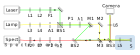
\includegraphics[width=\textwidth]{../figures/setup.jpg}
	\end{columns}
\end{frame}

\subsection{Transmission}
\begin{frame}{Raw measured relative Transmission}
	\begin{columns}
		\column{.6\textwidth}
		\centering
		\includegraphics[width=\textwidth]{../figures/2024-03-15 MnPS3 transmission raw.pdf}
		
		\column{.4\textwidth}
		$$T_{Relative} = \frac{T_\text{Sample}}{T_\text{Reference}}$$
		% \vspace{.5cm}
		\includegraphics[width=\textwidth]{../figures/carray schematic.png}\\
		\customcite{cary}
	\end{columns}
\end{frame}

\begin{frame}{Corrected Absorbance}
	\begin{columns}
		\column{.7\textwidth}
		MnPS$_3$ Absorbance with Photoluminescence:
		\begin{figure}
		% 	\centering
			\includegraphics[width=\textwidth]{../figures/2024-03-15 MnPS3 Absorbance with PL.pdf}
		\end{figure}

		\column{.3\textwidth}
		\begin{align*}
			T_{Relative} &= \frac{T_\text{Sample}}{T_\text{Reference}}\\
			T_{Measured} &= T_\text{R, Sample} \divisionsymbol T_\text{R, Hole}
		\end{align*}
	\end{columns}
\end{frame}
\begin{frame}{Different Samples}
	\begin{columns}
		\column{.7\textwidth}
		\centering
		\includegraphics[width=\textwidth]{../figures/2024-03-15 Absorbance.pdf}
		% Broad edge at the bandgap, therefore not

		\column{.3\textwidth}
		\centering
		\includegraphics[width=\textwidth]{../../photos/transmission holder.jpg}
		\includegraphics[width=\textwidth]{../../photos/transmission samples.jpg}
	\end{columns}
\end{frame}

\subsection{Reflection}
\begin{frame}{Setup for Reflection}
	\begin{columns}
		\column{.6\textwidth}
		\begin{figure}
			\centering
			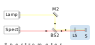
\includegraphics[width=\textwidth]{../figures/setup_reflection.pdf}
		\end{figure}
		
		\column{.4\textwidth}
		\begin{itemize}
			\item Polarizer {\color{seeblau}P$_1$} and Retarder {\color{seeblau}$\lambda_1$} remove excitation polarisation dependence
			\item Polarizer {\color{seeblau}P$_2$} and Retarder {\color{seeblau}$\lambda_2$} allow to detect different polarisations 
			\item Beamsplitter {\color{seeblau}BS$_2$} is a Polka-dot mirror to minimize the influence on polarisation
			\item Lens {\color{seeblau}L$_5$} has strong Chromatic Aberration
		\end{itemize}
	\end{columns}
\end{frame}

\begin{frame}{Reflection Spectra}

	\begin{columns}
		\column{.7\textwidth}
		\centering
		\includegraphics[width=\textwidth]{../figures/2024-03-14 reflection spectra.pdf}

		\column{.3\textwidth}
		Measured Spectra with broad shape from Halogen Lamp
		\vspace{.5cm}\\
		Reference using Mirror was difficult due to Chromatic Aberration of the last lens
	\end{columns}
\end{frame}

\begin{frame}{NiPS3: Reflection of bulk sample}
	\begin{columns}
		\column{.7\textwidth}
		\centering
		\includegraphics[width=\textwidth]{../figures/2024-02-06 NiPS3 PL and reflectance.pdf}

		\column{.3\textwidth}
		Thin film Interference below Bandgap, where the material is transparent
	\end{columns}
\end{frame}

\begin{frame}{Empirical Mode Decomposition}
	\begin{columns}
		\column{.6\textwidth}
		\centering
		\includegraphics[width=\textwidth]{../figures/2024-03-14 reflection spectra IMF.pdf}\\
		\scriptsize Idea for EMD: \customcite{thickness}

		\column{.4\textwidth}
		EMD $\sim$ Low Pass filter to Filter out Spectrum of Halogen Lamp 
	\end{columns}
\end{frame}

\begin{frame}{Thickness Estimation of Bulk Crystals}
	\begin{columns}
		\column{.5\textwidth}
		\centering
		\includegraphics[width=\textwidth]{../figures/2024-03-14 thickness .pdf}
		
		\column{.2\textwidth}
		\begin{figure}
			\centering
			\includegraphics[width=\textwidth]{../../data/2023-11-02/i001_MnPS3_50x_a.png}
			MnPS$_3$
		\end{figure}
		Different layers of cracks visible in a microscopy image

		\column{.3\textwidth}
		\begin{align*}
			R(\lambda) &= \cos 2 \pi \cdot 2 n d \cdot  \frac{1}{\lambda}\\
			\Rightarrow P_\nu(n d) &= \mathcal{F}\left[R\left(\frac{1}{\lambda}\right)\right]( 2 nd)\\
			&\approx  \mathcal{F}\left[\text{IMF}_1\; R\left(\frac{1}{\lambda}\right)\right]( 2 nd)\\
		\end{align*}
		$\mathcal{F}$: Lomb-Scargle method due to unevenly sampled data
	\end{columns}
\end{frame}

\begin{frame}{Reflection on exfoliated samples}
	\begin{columns}
		\column{.6\textwidth}
		\begin{figure}
			\centering
			$$R = \frac{R_\text{flake}}{R_\text{substrate}}$$\\
			\includegraphics[width=\textwidth]{../figures/2024-04-10 normalized reflection spectra.pdf}
		\end{figure}
		{\color{seeblau}$\Rightarrow$} 3 Interface Interference: Vacuum - Flake - SiO$_2$ - Si\\
		{\color{seeblau}$\Rightarrow$} Bandgap not visible
		
		\column{.4\textwidth}
		\begin{figure}
			\centering
			\includegraphics[width=\textwidth]{../figures/2024-03-14 thickness flakes.pdf}\\
		\end{figure}
		Extracted thickness matches with AFM measurements\\
		\vspace{1cm}
		\tiny
		Source for $n\sim1.5$: 		\fullcite{CrPS4_refrative}
	\end{columns}
\end{frame}

\subsection{Photoluminescence}
\begin{frame}{Setup for Photoluminescence}
	\begin{columns}
		\column{.6\textwidth}
		\begin{figure}
			\centering
			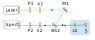
\includegraphics[width=\textwidth]{../figures/setup_simplified.pdf}
		\end{figure}
		
		\column{.4\textwidth}
		\begin{itemize}
			\item Polarizer {\color{seeblau}P$_1$} and Retarder {\color{seeblau}$\lambda_1$} remove excitation polarisation dependence
			\item Polarizer {\color{seeblau}P$_2$} and Retarder {\color{seeblau}$\lambda_2$} allow to detect different polarisations 
			\item Beamsplitter {\color{seeblau}BS$_2$} is a Polka-dot mirror to minimize the influence on polarisation
			\item Lens {\color{seeblau}L$_5$} has strong Chromatic Aberration
			\item Laser Wavelengths: 532 nm and 647 nm with up to 10 mW before L$_5$
		\end{itemize}
	\end{columns}
\end{frame}

\begin{frame}{Photoluminescence at 10K}
	\begin{columns}
		\column{.6\textwidth}
		\centering
		\includegraphics[width=\textwidth]{../figures/2023-12-10 Combined PL.pdf}

		\column{.4\textwidth}
		Expected splitting of the photoluminescence line\\
		$\Rightarrow$ the MnPS$_3$ peak is too broad
		\vspace{.5cm}\\
		Excited with 532 nm and 647 nm laser:\\
		no difference in main peak
		\vspace{.5cm}\\
		No degradation of the sample with up to 10 mW laser power
	\end{columns}
\end{frame}

\begin{frame}{Model for Photoluminescence}
	\begin{columns}
		\column{.5\textwidth}
		{\color{seeblau}Exciton Model:}
		\begin{itemize}
			% \item Excitons need $k_B T < E_\text{Binding}$ to 
			\item Bound electron-hole pair gets created by excitation photon $E> E_\text{Bandgap}$
			\item Exciton decays by phonon emission with $E_\text{Bandgap} - E_\text{Binding}$
			\item $E_\text{Binding}$ split with Zeeman effect
			\item Exciton has a magnetic moment\\ $\Rightarrow$ aligns with $B$ field\\ 
			$\Rightarrow$ linear polarisation if $M$ in-plane,\\
			 circ. polarisation if out-of-plane
		\end{itemize}

		\column{.5\textwidth}
		{\color{seeblau}Single Particle Model:}
		\begin{itemize}
			\item Field dependent (possibly complicated) band structure\\
			Can be calculated with DFT
			\item With some emitting transitions
			\item electron Spin dependent transitions \\$\Rightarrow$ Circular Polarisation  
		\end{itemize}
		\begin{figure}
			\centering
			\includegraphics[width=\textwidth]{../figures/CrPS4 bandstructure.png}
		\end{figure}
		\customcite{CrPS4_bandstructure}
	\end{columns}
\end{frame}

\subsection*{Summary}
\begin{frame}{Tried Techniques}
	\begin{tabular}{p{.3\textwidth} p{.3\textwidth} p{.3\textwidth}}
		\colorbox{seeblau}{Transmission} & \colorbox{seeblau}{Reflection} & \colorbox{seeblau}{Photo-Luminescence}\\

		\begin{itemize}
				\item large Sample Volume\\ $\Rightarrow$ strong Signal
				\item Technical Problems in the setup and not enough time to build a new one
		\end{itemize}&

		\begin{itemize}
			\item Multiple interferences in Flake and Si layer on Substrate
			\item Difficult to extract meaningful information
		\end{itemize}&

		\begin{itemize}
			\item strong enough signal
			\item sharp enough peak
			\item relatively easy to interpret
		\end{itemize}\\

		\begin{figure}
			\centering
			\includegraphics[width=.2\textwidth]{../figures/carray schematic.png}
		\end{figure}&
		\begin{figure}
			\centering
			\includegraphics[width=.3\textwidth]{../figures/2024-02-06 NiPS3 PL and reflectance.pdf}
		\end{figure}&
		\begin{figure}
			\centering
			\includegraphics[width=.2\textwidth]{../figures/2023-11-07 flake laser.jpg}
		\end{figure}

	\end{tabular}
\end{frame}


\section{Results}
\begin{frame}
	\begin{columns}
		\column{.4\textwidth}
		\tableofcontents[currentsection]

		\column{.4\textwidth}
		% \centering
		% \includegraphics[width=\textwidth]{../figures/2024-04-07 NiPS3 Splitting.pdf}
	\end{columns}
\end{frame}

\subsection{NiPS$_3$}
\begin{frame}{NiPS$_3$ Structure}
	\begin{columns}
		\column{.4\textwidth}
		\centering
		\includegraphics[width=\textwidth]{../../figures/crystal structures/NiPS3 structure.pdf}

		\column{.5\textwidth}
		Antiferromagnetic order\\
		\begin{figure}
			\centering
			\includegraphics[width=\textwidth]{../../figures/crystal structures/NiPS3 magnetic structure.pdf}
		\end{figure}
		Intra layer coupling $\gg$ Inter layer coupling\\
		Anisotropic Inter layer coupling
	\end{columns}
	\customcite{NiPS3_structure}	
\end{frame}

\begin{frame}{Splitting of the NiPS$_3$ Photoluminescence in one polarisation Direction}
	\begin{columns}
		\column{.7\textwidth}
		\begin{figure}
			\centering
			\includegraphics[width=\textwidth]{../figures/2024-04-07 NiPS3 Splitting.pdf}
		\end{figure}

		\column{.3\textwidth}
		The PL peak splits with magnetic Field.
		\vspace{.5cm}\\
		But by different amounts in different polarisation directions $P$ relative to the applied field $H$.
	\end{columns}
\end{frame}

\begin{frame}{Splitting already documented}
	\begin{columns}
		\column{.4\textwidth}
		The splitting was already observed, but without the polarisation measurement:
		\includegraphics[width=\textwidth]{splitting.png}
		\customcite{NiPS3_magnon_gap}

		\column{.6\textwidth}
		\begin{figure}
			\centering
			\includegraphics[width=\textwidth]{../figures/2024-04-07 NiPS3 Splitting.pdf}
		\end{figure}
	\end{columns}
\end{frame}

\begin{frame}{Fitting a simple model}
	\begin{columns}
		\column{.5\textwidth}
		{\color{seeblau}Simple Biaxial Antiferromagnet Model:}\\
		$\psi = \measuredangle(N, B)$\\
		$\theta_0 = \measuredangle(a, B) = \psi(B=0)$
		\begin{align*}
			\tan 2 \psi &= \frac{\sin 2 \theta_0}{\cos 2 \theta_0 - \frac{B}{B_{\text{SF}}}^2}\\
			\Delta E &= g \mu_B B \cos \psi
		\end{align*}
		\\\vfill
		\customcite{NiPS3_magnon_gap}
	
		\column{.5\textwidth}
		{\color{seeblau}Polarisation $\parallel$ Spin Alignment:}\\
		Neel Vector: $L = M_1 - M_2 \parallel \text{Spin Alignment}$\\
		$\psi = \measuredangle(L, B)$\\
		\includegraphics[width=\textwidth]{../figures/NiPS3 linear model.png}
		\customcite{NiPS3_linear}
	\end{columns}
\end{frame}

\begin{frame}{Fitting the Model}
	\begin{columns}
		\column{.6\textwidth}
		\includegraphics[width=\textwidth]{../figures/2024-04-07 NiPS3 Model.pdf}

		\column{.4\textwidth}
		\centering
		\includegraphics[width=\textwidth]{../figures/2024-04-07 NiPS3 polarisation.pdf}
	\end{columns}
	$\Rightarrow$ Model fits roughly
\end{frame}

\begin{frame}{The Model is too simple}
	\begin{columns}
		\column{.45\textwidth}
		{\color{seeblau}Different Splitting:}\\
		\includegraphics[width=\textwidth]{../figures/2024-04-09 NiPS3 model comparison.pdf}\\
		No difference in $\Delta E$ for different polarisations \\
		$\Rightarrow$ No difference in Splitting for different polarisations

		\column{.55\textwidth}
		{\color{seeblau}Polarisation:}\\
		Measurement:
		\includegraphics[width=\textwidth]{../figures/2024-04-09 NiPS3 polarisation Splitting.pdf}\\
		Model:
		\includegraphics[width=\textwidth]{../figures/2024-04-09 NiPS3 Model.pdf}
		No independent Polarisation for different Wavelengths
	\end{columns}
	\centering
	\highlight{
		$\Rightarrow$ Further Theorethical work is necessary
	}
\end{frame}




\subsection{CrPS$_4$}
\begin{frame}{Pl Circular Polarisation in Magnetic Field}
	\begin{columns}		
		\column{.55\textwidth}
		My measurement:\\
		\centering
		\includegraphics[width=\textwidth]{../figures/2023-12-14 CrPS4 circular dichroism.pdf}\\
		\raggedright
		\highlight{$\Rightarrow$ Circular Dichroism $\propto$ Magnetisation}\\
		$\Rightarrow$ Fast and Sensitive Measurement of Magnetisation in CrPS$_4$

		\column{.45\textwidth}
		\centering
		\includegraphics[width=\textwidth]{../notes/image14.png}
		\customcite{CrPS4_magnetic}
	\end{columns}
\end{frame}

\begin{frame}{Proof of Concept: Detecting Phase Transitions}
	\begin{columns}
		\column{.5\textwidth}
		\includegraphics[width=\textwidth]{../figures/2024-04-10 combined.pdf}
		
		\column{.3\textwidth}
		Spin-Flop at 10 K and .68 T,\\
		Spin-Flip at 7.5 T\\
		No Phase Transition at 50K\\
		{\color{seeblau}$\Rightarrow$} Demonstrates the using CD of the PL line to study Phase Transitions

		\column{.2\textwidth}
		\begin{figure}
			\centering
			\includegraphics[width=\textwidth]{../notes/phase_diagram_small.png}
			\includegraphics[width=.75\textwidth]{../notes/image1.png}\\
		\end{figure}
		\customcite{CrPS4_magnetic}

	\end{columns}
\end{frame}


\subsection{CrPS$_4$: Aligning Flakes}
\begin{frame}{Initial Measurements: Aligning CrPS$_4$ Flakes?}
	\begin{columns}
		\column{.5\textwidth}
		Photoluminescence Signal:
		{\centering
		\includegraphics[width=\textwidth]{../figures/2023-12-14 flake turning linear polarisation.pdf}}

		\column{.5\textwidth}
		\begin{figure}
			\centering
			\includegraphics[width=\textwidth]{../../data/2023-12-14_CrPS4_outPlane/flake03_rotation_cropped.png}
		\end{figure}
		Flake 03\\ \textbf{background}: flake after cooldown\\ \textbf{foreground}: flake before cooldown\\
		\vspace{.5cm}
		{\color{seeblau}$\Rightarrow$} Do the entire flakes align or just their PL polarisation?
	\end{columns}
\end{frame}

\begin{frame}{More Formal Measurement}
	\begin{columns}
		\column{.6\textwidth}
		\begin{figure}
			\centering
			\includegraphics[width=.8\textwidth]{../figures/2024-01-23 rotating pl.pdf}
			\includegraphics[width=\textwidth]{../figures/2024-01-23 flakes.pdf}\\
		\end{figure}
		\vfill
		\small
		Flake 03 and Flake 04-07 were on different misaligned substrates

		\column{.4\textwidth}
		Setup a better imaging system using dark field illumination.
		\vspace{.5cm}\\
		{\color{seeblau}$\Rightarrow$} polarisation aligns, but flakes do not rotate in the image.
		\vspace{.5cm}\\
		{\color{seeblau}$\Rightarrow$} Maybe the Si/SiO$_2$ substrate has something to do with it?
	\end{columns}
\end{frame}

\begin{frame}{Different Substrates}
	\begin{figure}
		\centering
		\includegraphics[width=\textwidth]{../figures/2024-01-29 rotating pl.pdf}
	\end{figure}
	{\color{seeblau}$\Rightarrow$} Not all flakes align, does not correlate with the size or position off the flakes\\
	{\color{seeblau}$\Rightarrow$} substrate independent\\
	{\color{seeblau}$\Rightarrow$} probably a variance in the sample preparation
\end{frame}


\begin{frame}{AFM Results of CrPS$_4$ flakes after cooldown on Si/SiO$_2$ and Glass Substrates}
	\begin{columns}
		\column{.6\textwidth}
		After Cooldown:\\
		\includegraphics[width=\textwidth]{../figures/2024-02-29 afm.pdf}
		\begin{figure}
			\centering
			\includegraphics[width=.5\textwidth]{../../data/2023-12-04_LO_MG_NiPS3/CrPS4_50x_10um.png}
			\\Scalebar 10$\mu$m
		\end{figure}

		\column{.4\textwidth}
		On the samples where all flakes aligned:\\ all flakes have a smooth \textit{"normal"} surface
		\vspace{.5cm}\\
		On the samples where not all flakes aligned:\\ some flakes have a rough surface
		\\ this rough patch is larger than the flakes on the substrate
		\vspace{.5cm}\\
		Thinner flakes appear to be torn by mechanical stress
		\vspace{.5cm}

	\end{columns}
\end{frame}


\begin{frame}{Possible Causes of the aligning Flakes}
	\begin{columns}
		\column{.5\textwidth}
		Ruled out causes:
		\begin{itemize}
			\item Residual Magnetic Field\\ The coil was turned out of plane $\Rightarrow$ no in plane torque on the flakes
			\item Inter flake forces\\ Different densities of the flakes were used, no significant correlation
			\item alignment due to exfoliation\\ The tape was rotated between each exfoliation step, the transfer to the substrate was done multiple, rotated times
		\end{itemize}

		\column{.5\textwidth}
		Follow up ideas:
		\begin{itemize}
			\item AFM images before cooldown: Is it already torn? Are the rough patches visible?
			\item Tape to Substrate transfer at a higher temperature: Are there more rough patches?
			\item Measure Direction using Polarized Raman, to minimize influence of strain. 
		\end{itemize}
	\end{columns}
\end{frame}

\section{Conclusion and Outlook}
\begin{frame}{Conclusion and Outlook}
	\begin{columns}
		\column{.6\textwidth}
		\begin{tabular}{p{.5\textwidth} p{.5\textwidth}}
			\colorbox{seeblau}{NiPS3} & \colorbox{seeblau}{CrPS4}\\

			\begin{itemize}
				\item Measured polarisation resolved splitting of the PL line
				\item Shown that current model does not fit the data\\$\Rightarrow$ more theoretical work needed
			\end{itemize}&

			\begin{itemize}
				\item Shown that CD of the PL line can be used to measure magnetisation, faster and more sensitive than previous methods
				\item[$\rightarrow$] More measurements are being taken today
				\item[$\rightarrow$] Noise measurements are planned
			\end{itemize}\\

			\begin{figure}
				\centering
				\includegraphics[width=.5\textwidth]{../figures/2024-04-07 NiPS3 Splitting.pdf}
			\end{figure}&
			\begin{figure}
				\centering
				\includegraphics[width=.5\textwidth]{../figures/2023-12-14 CrPS4 circular dichroism.pdf}
			\end{figure}\\
		\end{tabular}

		\column{.3\textwidth}
		{\color{seeblau}Side Projects:}
		\begin{itemize}
			\item Thickness Estimation:\\ Demonstrated a robust method for thickness estimation based on reflection spectra
			\item Rotating Flakes:\\ Observed mysterious alignment force
		\end{itemize}
	\end{columns}

\end{frame}



\section{Supplementary}
\begin{frame}
	\begin{columns}
		\column{.8\textwidth}
		\tableofcontents[currentsection]
	\end{columns}
\end{frame}

\begin{frame}{CrPS4: magnetic order}
	\begin{columns}
		\column{.6\textwidth}
		\fullgraphic{../notes/phase_diagram.png}
		\column{.15\textwidth}
		\fullgraphic{../notes/image1.png}
	\end{columns}
	\customcite{CrPS4_magnetic}
\end{frame}

\begin{frame}{Semiconductor Photoluminescence}
	\centering
	\includegraphics[scale=1.5]{../figures/Fig. 2 from Magneto-optical anisotropies of 2D antiferromagnetic MPX3 from first principles.pdf}\\
	\raggedleft \small
	Magneto-optical anisotropies of 2D antiferromagnetic MPX3 from first principles, arXiv 2023
\end{frame}

\begin{frame}{Full Setup}
		\begin{figure}
			\centering
			\includegraphics[width=\textwidth]{../figures/setup.pdf}
		\end{figure}
\end{frame}

\begin{frame}{NiPS$_3$: Model Problems}
	\begin{columns}
		\column{.5\textwidth}
		\includegraphics[width=\textwidth]{../figures/2024-04-07 NiPS3 Model Fit Problem.pdf}

		\column{.5\textwidth}
		\centering
		\includegraphics[width=\textwidth]{../figures/2024-04-07 NiPS3 polarisation Problem.pdf}
	\end{columns}
	
	\customcite{NiPS3_magnon_gap}\\
	\fullcite{NiPS3_linear}
\end{frame}

\begin{frame}{Magnitude of Spectra is unstable}
	\begin{columns}
		\column{.6\textwidth}
		\centering
		\includegraphics[width=\textwidth]{../figures/2023-12-10 lens movement.pdf}
		NiPS3, magnitude of photoluminescence peak

		\column{.3\textwidth}
		\begin{figure}
			\centering
			\includegraphics[width=\textwidth]{../figures/sampleHolder.pdf}
			Field in plane of the image.
		\end{figure}
	\end{columns}
\end{frame}

\begin{frame}{CrPS4}
	linear Polarisation, 10 K, in-plane field:
	\includegraphics[width=\textwidth]{../figures/2024-04-09 CrPS4 linear Polarisation.pdf}
\end{frame}

\begin{frame}{Flakes NiPS3, based on Raman signal}
	\includegraphics[width=\textwidth]{../figures/2024-01-03 NiPS3 flake rotation.pdf}
\end{frame}

\begin{frame}{NiPS3 magneto raman}
	\includegraphics[width=\textwidth]{NiPS3 magnet raman.png}
\end{frame}


\end{document}